\chapter{Implementation}

Stuff to insert:
\begin{itemize}
	\item Generation of random points
	\item Noise generation on GPU
	\item Sampling patterns
	\item Layered rendering
	\item Shadow mapping (for lights)
	\item Ping ponging and accumulation
	\item Texture Views and mipmap generation (memory optimization)
	\item Engine structure
	\item Extension: compute shaders
	\item Extension: image load store
	\item Extension: subroutines (meh)
	\item Sampling cubemap

\end{itemize}

Caveats:
\begin{itemize}
	\item Oversampling issues in final combinaiton (multisampling of depth map)
	\item Combination delta
	\item Shadow bias
  \item Random rotation
	
\end{itemize}

\begin{lstlisting}[language=GLSL,label=test,caption=Test!]
#version 430
layout(triangles) in;
layout(triangle_strip, max_vertices = 60) out;

#include "ss_aincludes_constants.glinc"

uniform int layers;
uniform mat4 P;
uniform mat4 viewMatrices[DIRECTIONS];

smooth in vec3 v_position[3];
smooth in vec3 v_norm[3];

smooth out vec3 position;
smooth out vec3 norm;

void main(void)
{
    int l = layers;
    for(int i = 0; i < l; i++)
    {
        gl_Layer = i;

        for(int k = 0; k < 3; k++)
        {
            vec4 v0 = gl_in[k].gl_Position;
            position = v_position[k];
            norm = v_norm[k];
            gl_Position = P * viewMatrices[i] * v0;
            EmitVertex();
        }

        EndPrimitive();
    }
}
\end{lstlisting}

In this chapter, we describe the implementation details of our technique, using the approximation of the rendering equation introduced in the previous chapter. We start by giving a rather generic introduction of our algorithm, introducing then all the implementation details. 

\section{Requirements}

Our algorithm, in order to be generic and applicable to a wide range of situations must meet some requirements. 


\begin{itemize}
  \item The algorithm should be \emph{accurate}, so that the renderings are as close as possible to reference images generated using a offline Monte-Carlo simulation. 
	\item The algorithm should be \emph{fast}, executing at interactive frame rates.
	\item The algorithm should be \emph{uv-independent}, not relying on a pre-made UV mapping of the object in order to being able to perform. The algorithm should work only if basic geometric features are provided (vertices and normals).
	\item The algorithm should be \emph{adaptable}, handling in real-time dynamic light changes and object deformations. So it will not possible to use light baking or geometry form factors.
\end{itemize}

If it is not possible to satisfy all the previous within the strict constraints of real-time rendering, we want to create an algorithm that gets as close as possible to the requested result. The algorithm should progressively progressively improve and converge to an accurate result whenever possible (e.g. when the light in the scene is not changing).

\section{Algorithm overview}

By keeping the limitations presented in the previous section in mind, we introduce our four pass algorithm.

\textbf{Step 1 - Light buffer} \\
In the first step, positions and normals of the object are rendered into a texture from the light point of view. In addition, for each light a conversion matrix is computed and stored, in order to convert the position from world space to texture space. 

\begin{figure}[!ht]
\centering
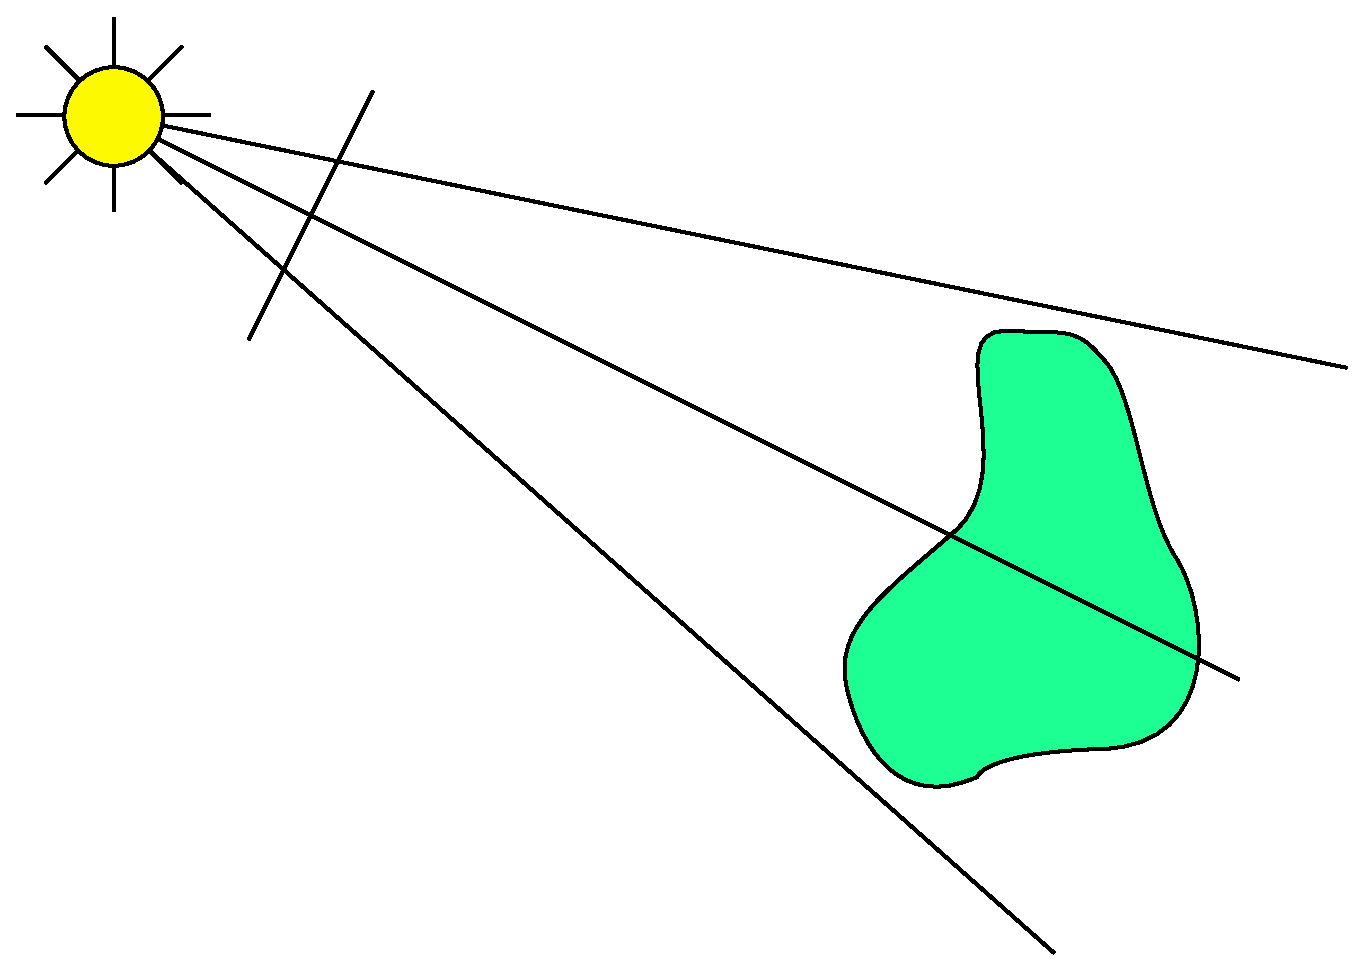
\includegraphics[width=0.5 \linewidth]{images/method/step1}
\caption{Render to G-buffer.}
\label{fig:step1}
\end{figure} 


\textbf{Step 2 - Render to array texture} \\
In the second step, we render the object from different directions into an array texture. Each layer of the texture represents a direction from which the object is rendered to. If we are able to cover all the surface of the model, 
Since the BSSRDF model we are using is view-independent (apart from a Fresnel term) we can combine the results of the cubemap in a final combination step.

\begin{figure}[!ht]
\centering
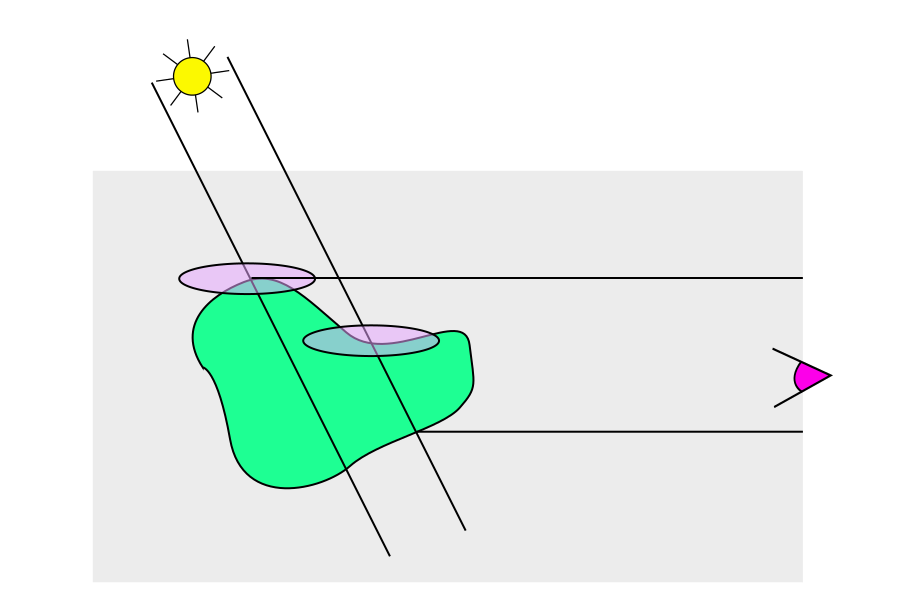
\includegraphics[width=0.5 \linewidth]{images/method/step2}
\caption{Render to cubemap.}
\label{fig:step2}
\end{figure} 

When we are rendering a point from the orthographic camera that represents a side of the cubemap, we do as illustrated in Figure \ref{fig:stepfrustum}. For each fragment, we calculate the closest point to the light, sampling the texture calculated in the previous step. In Figure  \ref{fig:stepfrustum} we have two examples, of when the two points coincide (directly lit) and when the two points does not (light passing through the object). 

\begin{figure}[!ht]
\centering
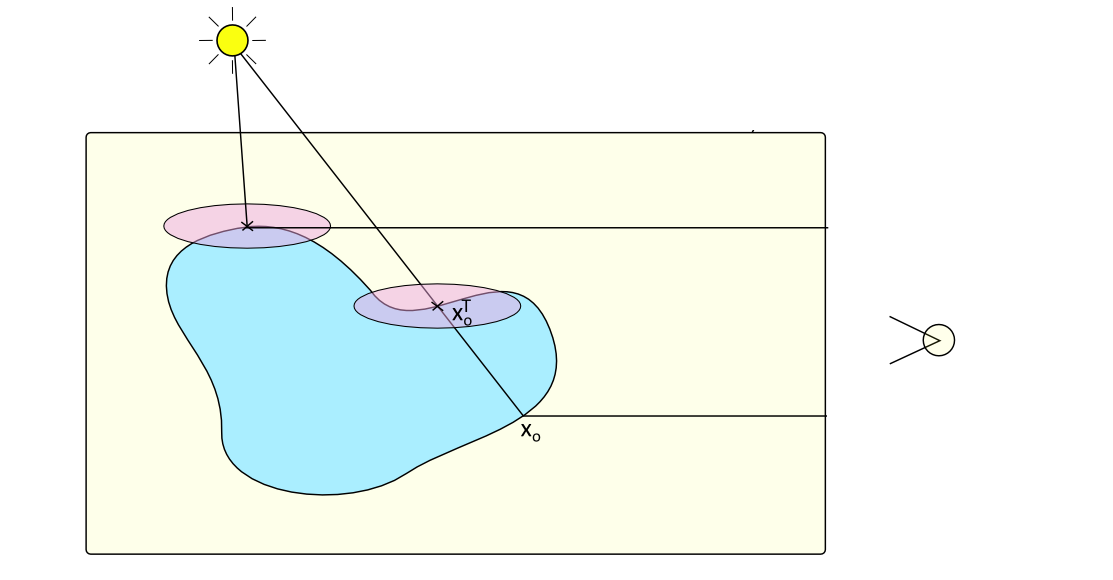
\includegraphics[width=\linewidth]{images/method/method_frustumside}
\caption{Render to cubemap, side view. Note that the fragment $\mathbf{x}^T_o$ is not rendered in this step, but only the point $\mathbf{x}_o$ is.}
\label{fig:stepfrustum}
\end{figure} 


Then, we place a disk in the texture and accumulate the BSSRDF from the neighboring points, as shown in Figure \ref{fig:stepgbuffer}. The points are chosen on the disk according to a pre-determined sampling scheme (discussed later). In order to accumulate the points and perform the right area integral, we need to assume that all the points on the disk cover the same area. So, we accumulate the point according to this formula:


\[
C^f(\mathbf{x}_o) = \sum_{i = 1}^{k} L_i(\mathbf{x}_i,\vec{\mathbf{\omega}}_i) S_i(\mathbf{x}_i,\mathbf{x}_o,\vec{\mathbf{\omega}}_i, \vec{\mathbf{\omega}}_o) \; (\vec{n_i}\cdot \vec{\mathbf{\omega}}_i) \; F_t(\vec{n_i},\vec{\mathbf{\omega}}_i) 
\]

where $\mathbf{x}_o$ is the exiting point $C^f$ is the cubemap on face $f$, $L_i$ is the incoming radiance, $S_i$ is the BSSRDF, $\mathbf{x}_i$ and $\vec{n_i}$ are the position and the normal sampled from a point of the disc, $k$ is the number of samples, and $F_t$ is the incoming Fresnel term.

\begin{figure}[!ht]
\centering
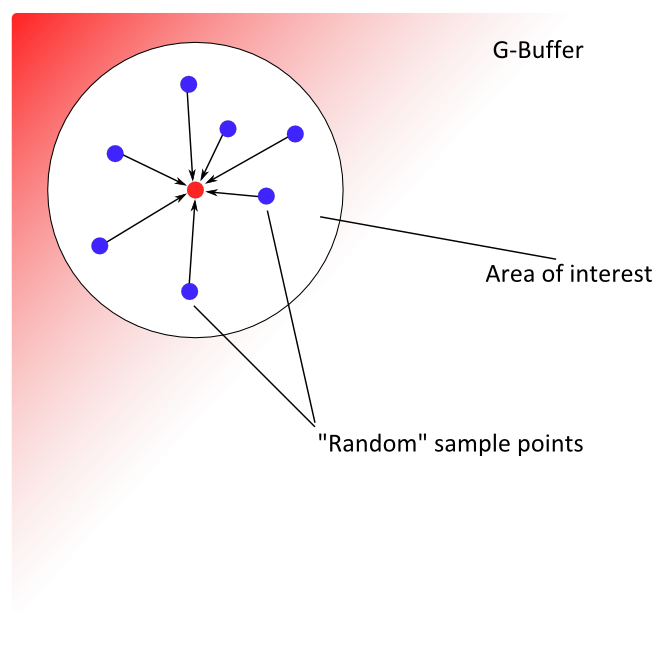
\includegraphics[width=0.5 \linewidth]{images/method/method_gbuffer}
\caption{Render to cubemap, gbuffer view.}
\label{fig:stepgbuffer}
\end{figure} 

\FloatBarrier
\textbf{Step 3 - Combination} \\
In this step, for each fragment on the surface we sample all the six cubemap sides as illustrated in Figure \ref{fig:step3}. In order to do this, we need a depth cubemap that inform us if the fragment was visible when we rendered the cubemap face. Then, each point is divided by the number of visible faces to average it. In formulas, to get the final luminance:

$$
L(\mathbf{x}) = \frac{\sum_{i = 1}^{6}V_{i}C(\mathbf{x}_{proj}^i)}{\sum_{i = 1}^{6}V_{i}}
$$

where $V_{i}$ is a visibility function that is zero if the point is not visible on the face $i$ and 1 if it is visible. $C(\mathbf{x})$ is the sample from the cubamap obtained in the previous step, and $\mathbf{x}_{proj}^i$ is the point $\mathbf{x}$ projected on the $i$-th cubemap face.

\begin{figure}[!ht]
\centering
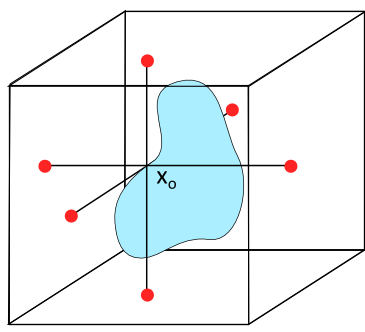
\includegraphics[width=0.5 \linewidth]{images/method/method_step3}
\caption{Final combination step. Note that the point is generally not visible from all the cubemap faces.}
\label{fig:step3}
\end{figure} 

\clearpage
\section{Implementation details}

\section{Artifacts}
A simple implementation of the method described until now is not completely correct. In fact, since we are discretizing the surface on a texture, some sampling artifacts are inevitable. During our implementation we identified three different types of artifacts:

\begin{itemize}
	\item Incorrect sampling of the G-buffer
	\item Incorrect sampling of the cubemap
	\item Shadow bias (when sampling the depth of the texture).
\end{itemize}

That are described in detail in the following sections.

\subsection{Incorrect sampling of the G-buffer}

In order to sample the G-buffer correctly, we need to modify the world coordinate of the point $\mathbf{x}_o$ with normal $\vec{n}_o$ in order to "shrink" a little bit towards the inside of the object according to the light direction $\vec{\omega}_l$:

$$
\mathbf{x}_o' = \mathbf{x}_o - \epsilon_g (\vec{n}_o - \vec{\omega}_l ( \vec{\omega}_l \cdot  \vec{n}_o))
$$

\subsection{Incorrect sampling of the cubemap}

Since we are sampling a cubemap, we do not need to account for the light direction in this case. In addition, the cubemap needs a 3D vector to be sampled with. So, instead of using $\mathbf{x}_o$, we use a point slightly intruded (i.e. displaced along the normal) in the calculations, according to:

$$
\mathbf{x}_o' = \mathbf{x}_o - \epsilon_c \vec{n}_o
$$

\subsection{Shadow bias}

In order to avoid artifacts such as shadows acne, we use a bias when comparing the z values of a point to determine if the point is in shadow or not. This implies that we need to convert the depth value from texture space ($\mathbf{z}_{tex}$) to world space again ($\mathbf{z}_{world}$). Since we are using an orthographics camera, the z value is the same in clip coordinates and in normalized device coordinates. Then, we simply use the camera projection properties ($\mathbf{z}_{far}$, $\mathbf{z}_{near}$) to convert the depth into the camera local space, in order to finally add the camera position transformed z value ($\mathbf{z}_{camera}$) and reconstruct the depth in world space:

$$
\mathbf{z}_{world} = \mathbf{z}_{camera} - \frac{\mathbf{z}_{far} - \mathbf{z}_{near}}{2} \left( 2 \mathbf{z}_{tex} - 1 + \frac{\mathbf{z}_{far} + \mathbf{z}_{near}}{\mathbf{z}_{far} - \mathbf{z}_{near}}\right)
$$
		
And finally compare the obtained z with the z position in world space of the point ($\mathbf{z}$) using the bias $\epsilon_b$, so a point is lit iff:

$$
\mathbf{z}_{world} - \epsilon_b < \mathbf{z}
$$		

\begin{figure}
\centering
\subfloat[Without shadow bias and sampling fixes]{
  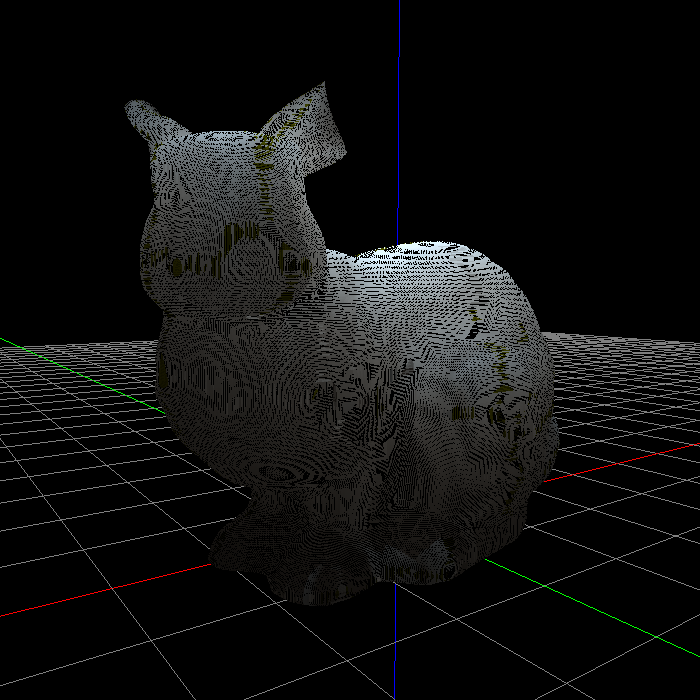
\includegraphics[width=0.45 \linewidth]{images/artifacts/all}
  \label{fig:art_ss1}
} 
\subfloat[With shadow bias and without sampling fixes]{
  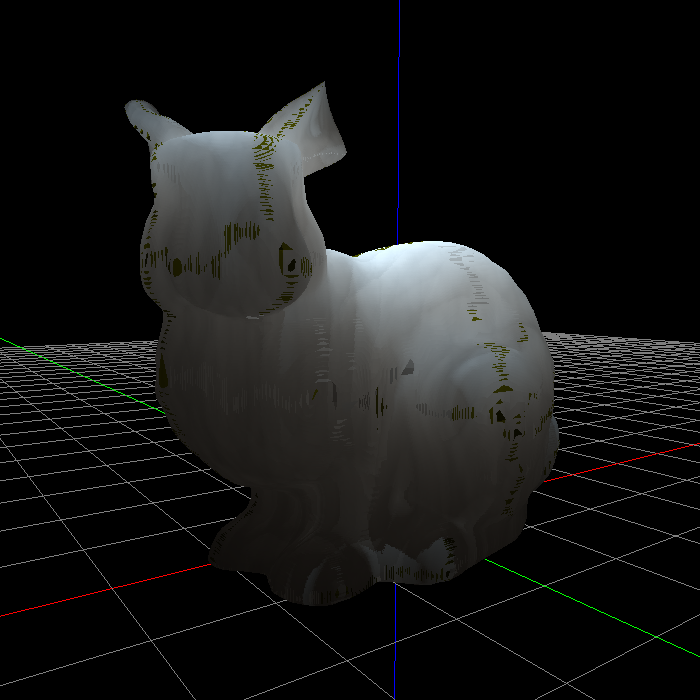
\includegraphics[width=0.45 \linewidth]{images/artifacts/nobias}
  \label{fig:art_ss2}
} 
\\
\subfloat[With both shadow bias and sampling fixes]{
  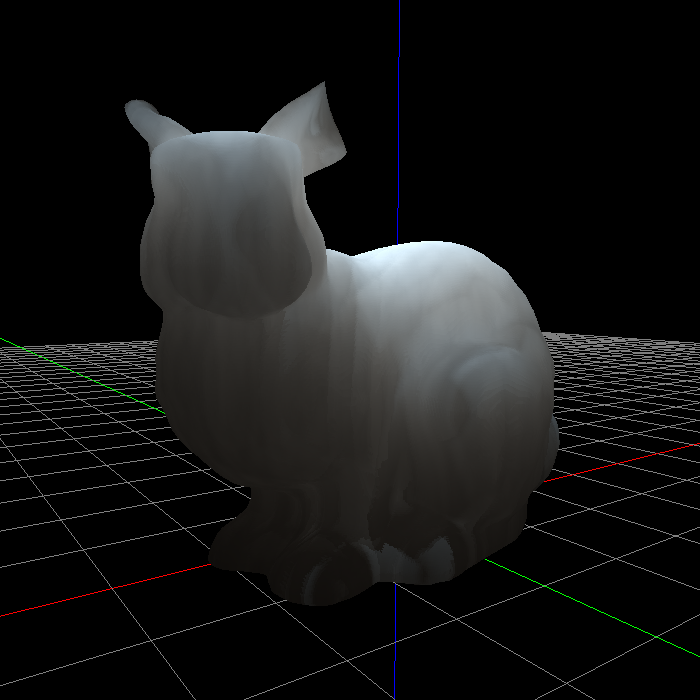
\includegraphics[width=0.45 \linewidth]{images/artifacts/cmboffset}
  \label{fig:art_ss3}
}
\subfloat[Reference]{
  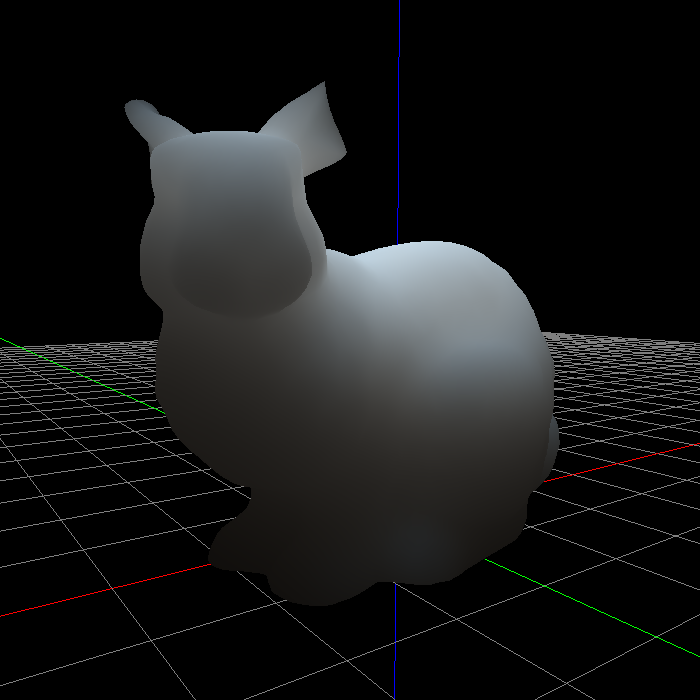
\includegraphics[width=0.45 \linewidth]{images/artifacts/reference}
  \label{fig:art_ss4}
}
\caption{Progressively removing artifacts to get to the final image. }
\label{fig:artifacts}
\end{figure} 
